\documentclass[conference]{IEEEtran}
\usepackage{cite}
\usepackage{amsmath,amssymb}
\usepackage{graphicx}
\usepackage{booktabs}
\usepackage{url}
\usepackage[T1]{fontenc}
\usepackage{textcomp}
\graphicspath{{../results/figures/}}
\hyphenation{Bayes-ian}

\begin{document}

\title{Heart Disease Risk Modelling, Phase~1:\\Bayesian Networks and Classical Baselines\\on the UCI Cleveland Data}

\author{
\IEEEauthorblockN{Aaryan Yadav}
\IEEEauthorblockA{2401010011\\aaryan.yadav2024@nst.rishihood.edu.in}
\and
\IEEEauthorblockN{Shivam Mishra}
\IEEEauthorblockA{2401010442\\shivam.mishra2024@nst.rishihood.edu.in}
\and
\IEEEauthorblockN{Satyam Kumar}
\IEEEauthorblockA{2401010429\\satyam.kumars2024@nst.rishihood.edu.in}
\and
\IEEEauthorblockN{Himank Kaushik}
\IEEEauthorblockA{2401010187\\himank.kaushik2024@nst.rishihood.edu.in}
\and
\IEEEauthorblockN{Mohammed Yaseen}
\IEEEauthorblockA{2401010281\\mohammed.yaseen2024@nst.rishihood.edu.in}
\\[1ex]
\IEEEauthorblockA{Advanced Machine Learning, Project 15 (Phase 1: classical machine learning)}
}

\maketitle

\begin{abstract}
We compare a hand-specified discrete Bayesian network (BN) with discrete Naive Bayes (NB), regularised logistic regression and a random forest on the 303-row UCI processed Cleveland data. The target is existing angiographic disease status ($\mathrm{num}>0$). All models share 25 stratified cross-validation splits (5 folds $\times$ 5 repeats). Out-of-fold ROC AUC lies between 0.896 (BN) and 0.911 (continuous logistic regression); none of the exploratory paired AUC comparisons detected a difference, which does not establish equivalence. Probability quality differs more clearly: calibration slopes are 0.51 (NB), 0.49 (BN), 0.98 (logistic regression) and 1.42 (random forest). A matched continuous heart-rate control separates binning from a change of feature representation. We document the graph, the discretisation cut points, missing-data handling, an exact additive explanation of the BN posterior, and the limitations of a small single-centre sample. This is a prediction exercise, not clinical decision support. The neural network and SHAP analysis belong to Phase~2 and are not part of this report.
\end{abstract}

\begin{IEEEkeywords}
Bayesian networks, Naive Bayes, calibration, heart disease, cross-validation, probabilistic classification
\end{IEEEkeywords}

%% ------------------------------------------------------------------------------------
\section{Introduction}
Predicting disease from patient records is usually judged by how well a model \emph{ranks} patients, yet a probability is only useful if it can be read as a probability. This project contrasts two ways of building such a model. The first writes down the dependence structure from domain knowledge (a Bayesian network); the second learns whatever the data supports (logistic regression, forests and, in Phase~2, a neural network).

The project brief frames a ``gap'': a fixed graph and coarse discretisation may miss continuous and nonlinear interactions among age, heart rate, blood pressure and symptoms. Phase~1 (this report) covers exploratory data analysis, the discretised Bayesian models and classical baselines. Phase~2 will add a regularised multilayer perceptron (MLP) and SHAP-based comparison. We test three hypotheses, each stated so that it can fail:
\begin{itemize}
\item \textbf{H1 (discretisation):} replacing continuous inputs by clinically motivated bins loses ranking information.
\item \textbf{H2 (structure):} the domain-informed BN outperforms Naive Bayes, and an interaction-capable learner (random forest) outperforms an additive one (logistic regression).
\item \textbf{H3 (probabilities):} model families differ in calibration, not only in ranking.
\end{itemize}
\emph{Scope and safety.} The label is existing angiographic disease status in a 1980s research cohort, not future risk. Nothing here is a medical recommendation.

%% ------------------------------------------------------------------------------------
\section{Related Work and Background}
\textbf{The data.} The Cleveland subset of the UCI Heart Disease repository \cite{janosi1989uci} comes from a multi-site study of a probability algorithm for diagnosing coronary artery disease \cite{detrano1989}; the Cleveland file is the one most commonly used for machine learning. Its small size and single-centre origin shape every conclusion below.

\textbf{Bayesian networks.} A BN encodes a joint distribution as a product of local conditional distributions over a directed acyclic graph \cite{pearl1988}. Used as a classifier, the class node is queried given the observed findings by exact inference. When the graph comes from experts and only the tables are estimated, BDe/BDeu priors give a principled way to smooth sparse counts \cite{heckerman1995}. Friedman et~al.\ \cite{friedman1997} compared Naive Bayes with richer network classifiers and showed that allowing limited dependencies between attributes can help, but that general networks learned with a likelihood-based score do not always beat Naive Bayes on classification. Our graph is hand-specified rather than learned, so we test the expert-structure case directly. The pgmpy library \cite{ankan2015} provides the estimator and inference used here.

\textbf{Naive Bayes.} Domingos and Pazzani \cite{domingos1997} showed that Naive Bayes can classify well even when its independence assumption is badly violated, because classification only needs the correct class to receive the highest probability, not for the probabilities themselves to be accurate. This predicts our observation that NB ranks as well as the other models but produces extreme probabilities.

\textbf{Calibration.} Niculescu-Mizil and Caruana \cite{niculescu2005} found that Naive Bayes pushes predicted probabilities towards 0 and~1, that logistic regression is usually well calibrated, and that bagged trees and random forests tend to be pulled away from the extremes. Guo et~al.\ \cite{guo2017} showed that modern neural networks are often over-confident, which motivates measuring calibration \emph{before} the Phase~2 network is built. In clinical prediction, the calibration slope and intercept and reliability plots are standard diagnostics \cite{steyerberg2010,vancalster2019}; expected calibration error (ECE) is a binned summary \cite{naeini2015}; the Brier score \cite{brier1950} measures overall probability error and mixes calibration with discrimination.

\textbf{Evaluation.} Precision--recall summaries are most informative under strong class imbalance \cite{saito2015}; our data are close to balanced (45.9\% positive), so average precision (AP) and ROC AUC carry similar information here. Repeated cross-validation produces overlapping training sets, which makes naive paired $t$-tests anti-conservative; Nadeau and Bengio \cite{nadeau2003} propose a corrected resampled $t$-test, and Dietterich \cite{dietterich1998} reviews the pitfalls of comparing classifiers with limited data. We follow reporting guidance for prediction models \cite{collins2015} where it applies to a course exercise.

\textbf{Position of this work.} We do not propose a new method. We apply expert-structure BNs, NB and baselines under one leak-free protocol, add a control that separates two confounded factors (binning versus feature engineering), and report calibration and uncertainty honestly. Phase~2 will add the MLP \cite{guo2017} and SHAP \cite{lundberg2017}.

%% ------------------------------------------------------------------------------------
\section{Dataset and Exploratory Analysis}
\subsection{Source and target}
We use only \texttt{processed.cleveland.data} from the official UCI archive: 303 patients, 13 predictors and the original label $\mathrm{num}\in\{0,\dots,4\}$ with counts 164, 55, 36, 35, 13. The file was verified byte-for-byte against the official ZIP (SHA-256 recorded in the repository). The binary target is $y=\mathbb{1}[\mathrm{num}>0]$, giving 139 positives and 164 negatives (45.9\% positive); $\mathrm{num}$ is never a predictor. Numeric predictors are age, resting blood pressure (\texttt{trestbps}), cholesterol (\texttt{chol}), maximum heart rate (\texttt{thalach}) and ST depression (\texttt{oldpeak}). Categorical predictors are \texttt{sex}, chest-pain type (\texttt{cp}), fasting sugar (\texttt{fbs}), resting ECG (\texttt{restecg}), exercise angina (\texttt{exang}), ST slope (\texttt{slope}), coloured vessel count (\texttt{ca}) and thallium scan (\texttt{thal}).

\subsection{What the data show}
Missing values are \texttt{?} in the source: \texttt{ca} has four and \texttt{thal} two, affecting six rows. There are 206 male and 97 female rows; disease prevalence is 55\% in men and 26\% in women. Asymptomatic chest pain ($\mathrm{cp}=4$, $n=144$) has 73\% disease; $\mathrm{ca}=0$ ($n=176$) has 26\% versus 68--85\% for $\mathrm{ca}\ge 1$. Patients with disease are older (mean 56.6 vs.\ 52.6 years), reach a lower maximum heart rate (139 vs.\ 158 bpm) and have more ST depression (1.57 vs.\ 0.59). Maximum heart rate falls with age (Spearman $\rho=-0.39$) and blood pressure rises with age ($\rho=+0.29$) (Fig.~\ref{fig:corr}). Univariate ROC AUC is highest for \texttt{thalach} (0.745, inverted) and \texttt{oldpeak} (0.735). No exact duplicate predictor rows exist, but the processed file has no patient identifiers, so row independence is an assumption. Category-level rates are shown in Fig.~\ref{fig:cat}. Associations are not causal effects.

\begin{figure*}[!t]
\centering
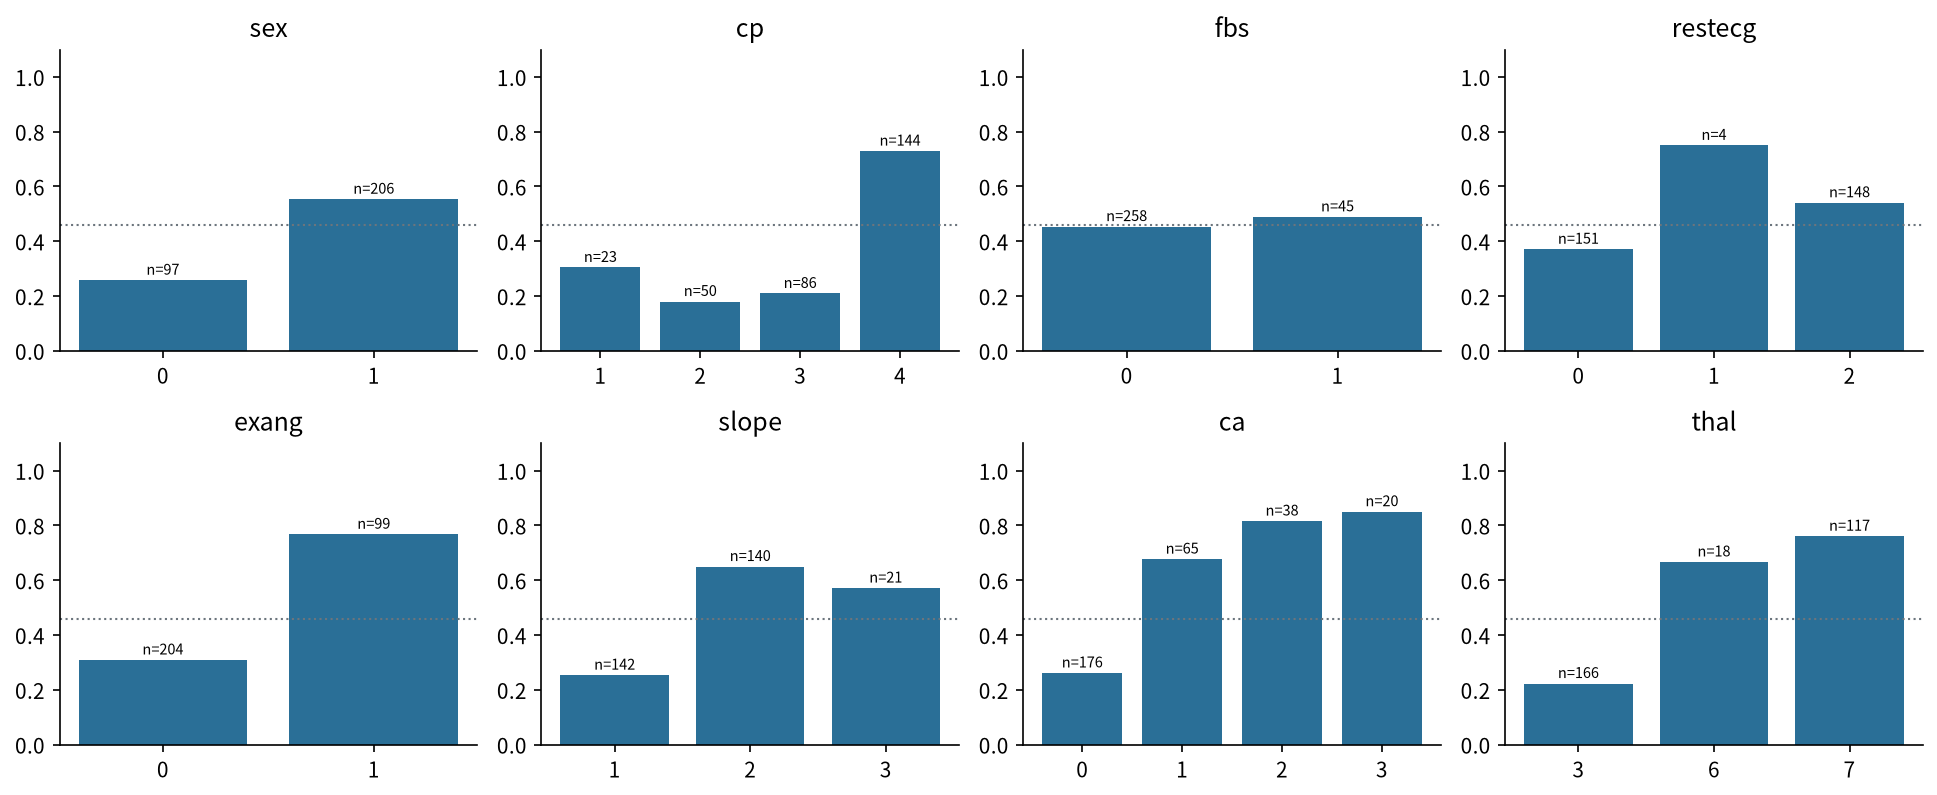
\includegraphics[width=0.78\textwidth]{fig_eda_categorical.png}
\caption{Disease rate by category with sample counts; dotted line is overall prevalence. Small categories (e.g.\ \texttt{restecg}=1, $n=4$) give unstable rates.}
\label{fig:cat}
\end{figure*}

\begin{figure*}[!t]
\centering
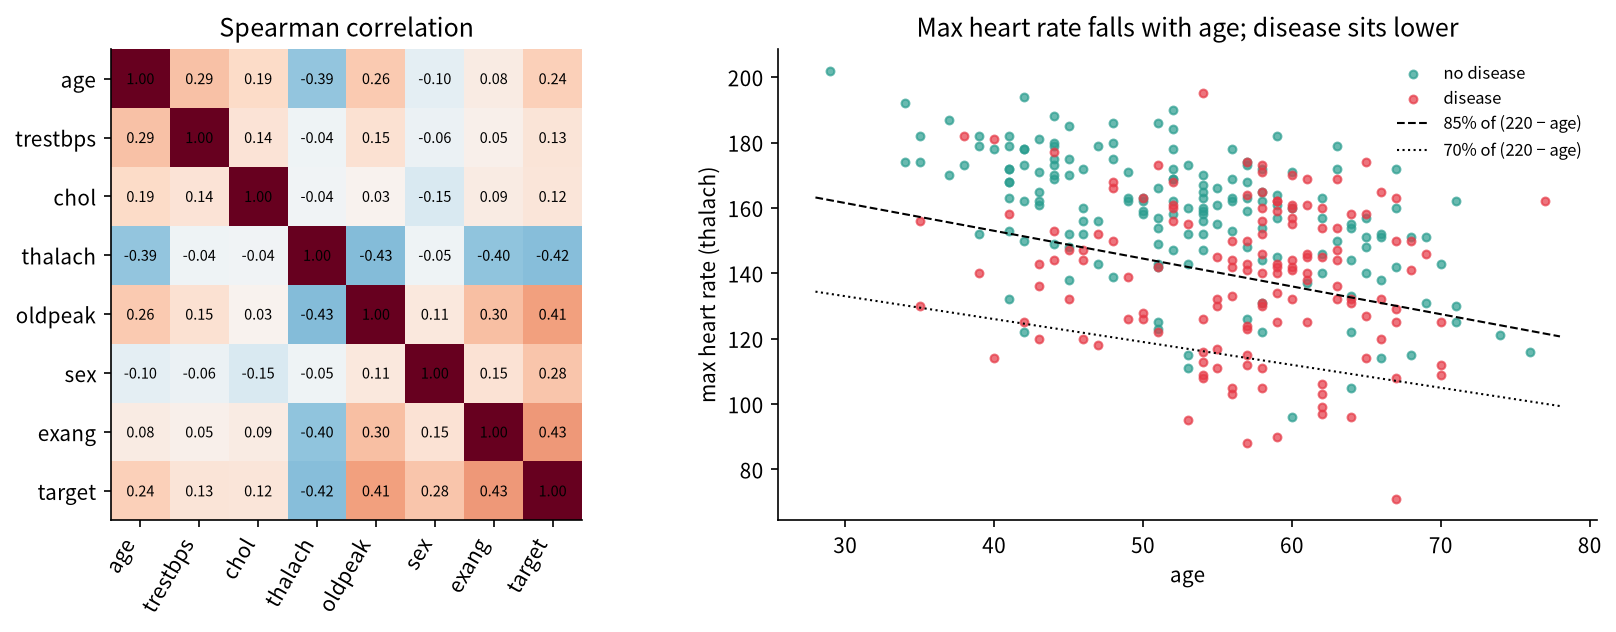
\includegraphics[width=0.78\textwidth]{fig_eda_corr_hr.png}
\caption{Left: Spearman correlations. Right: maximum heart rate against age, with 70\% and 85\% of $(220-\mathrm{age})$ marked. This relationship motivates the age-adjusted heart-rate feature and the age$\rightarrow$BP edge.}
\label{fig:corr}
\end{figure*}

%% ------------------------------------------------------------------------------------
\section{Feature Engineering and Preprocessing}
\textbf{Discretisation.} Bayesian models need discrete states. Cut points are fixed constants, not fitted on validation data, and are modelling choices rather than validated diagnostic rules (Table~\ref{tab:cuts}). Bins are right-open $[a,b)$. Heart rate is engineered as $\mathrm{apmhr}=\mathrm{thalach}/(220-\mathrm{age})$, the fraction of the age-predicted maximum achieved, because raw heart rate is confounded with age (Fig.~\ref{fig:corr}).

\begin{table}[!t]
\caption{Discretisation cut points (fixed modelling constants)}
\label{tab:cuts}
\centering
\begin{tabular}{lll}
\toprule
Variable & Interior cut points & States \\
\midrule
age & 50, 60 & $<$50, 50--59, $\ge$60 \\
trestbps & 130 & $<$130, $\ge$130 \\
chol & 240 & $<$240, $\ge$240 \\
apmhr & 0.70, 0.85 & $<$70\%, 70--84\%, $\ge$85\% \\
oldpeak & 1, 2 & $<$1, 1--$<$2, $\ge$2 \\
\bottomrule
\end{tabular}
\end{table}

\textbf{Missing data and encoding.} For continuous-input models, median (numeric) and most-frequent (categorical) imputation, standardisation and one-hot encoding are fitted on the training folds only. Categorical state spaces come from the UCI codebook, so unseen categories cannot break a fold. For Bayesian models, missing values are retained: each conditional table is estimated from locally available counts (not EM), and at prediction time missing evidence is simply omitted so exact inference marginalises it. If missingness is informative this introduces bias; with six affected rows the effect is probably small but is not measured.

\textbf{Design caveat.} Parts of the graph and the heart-rate transform were motivated by the full-data EDA above. This is exploratory model development, not a preregistered confirmatory study, so some optimism is possible.

%% ------------------------------------------------------------------------------------
\section{Models and Theory}
\subsection{Bayesian network classifier}
Let $Y\in\{0,1\}$ be disease status and $\mathbf{X}$ the discretised predictors. A BN factorises the joint as
\begin{equation}
P(Y,\mathbf{X})=\prod_{v\in\{Y\}\cup\mathbf{X}} P\bigl(v\mid \mathrm{pa}(v)\bigr).
\end{equation}
Our hand-specified graph (Fig.~\ref{fig:bn}) has 14 nodes and 16 edges: risk factors (age, sex, \texttt{trestbps}, \texttt{chol}, \texttt{fbs}) $\rightarrow Y$; $Y\rightarrow$ findings (\texttt{cp}, \texttt{exang}, \texttt{oldpeak}, \texttt{slope}, \texttt{restecg}, \texttt{apmhr}, \texttt{ca}, \texttt{thal}); plus age$\rightarrow$\texttt{trestbps}, \texttt{exang}$\rightarrow$\texttt{cp} and \texttt{oldpeak}$\rightarrow$\texttt{slope}. Arrows are modelling assumptions, not established causal relations. Disease has five parents, hence $3\cdot2\cdot2\cdot2\cdot2=48$ parent configurations for about 242 training rows per fold, so its table is sparse and smoothing matters.

Parameters use a Bayesian estimate with a BDeu prior with equivalent sample size $\alpha=5$ \cite{heckerman1995}. For node $i$ with $r_i$ states, $q_i$ parent configurations and counts $N_{ijk}$,
\begin{equation}
\hat\theta_{ijk}=\frac{N_{ijk}+\alpha/(r_i q_i)}{N_{ij}+\alpha/q_i}.
\end{equation}
Prediction is exact inference by variable elimination for $P(Y{=}1\mid\mathbf{x}_{\mathrm{obs}})$.

\begin{figure}[!t]
\centering
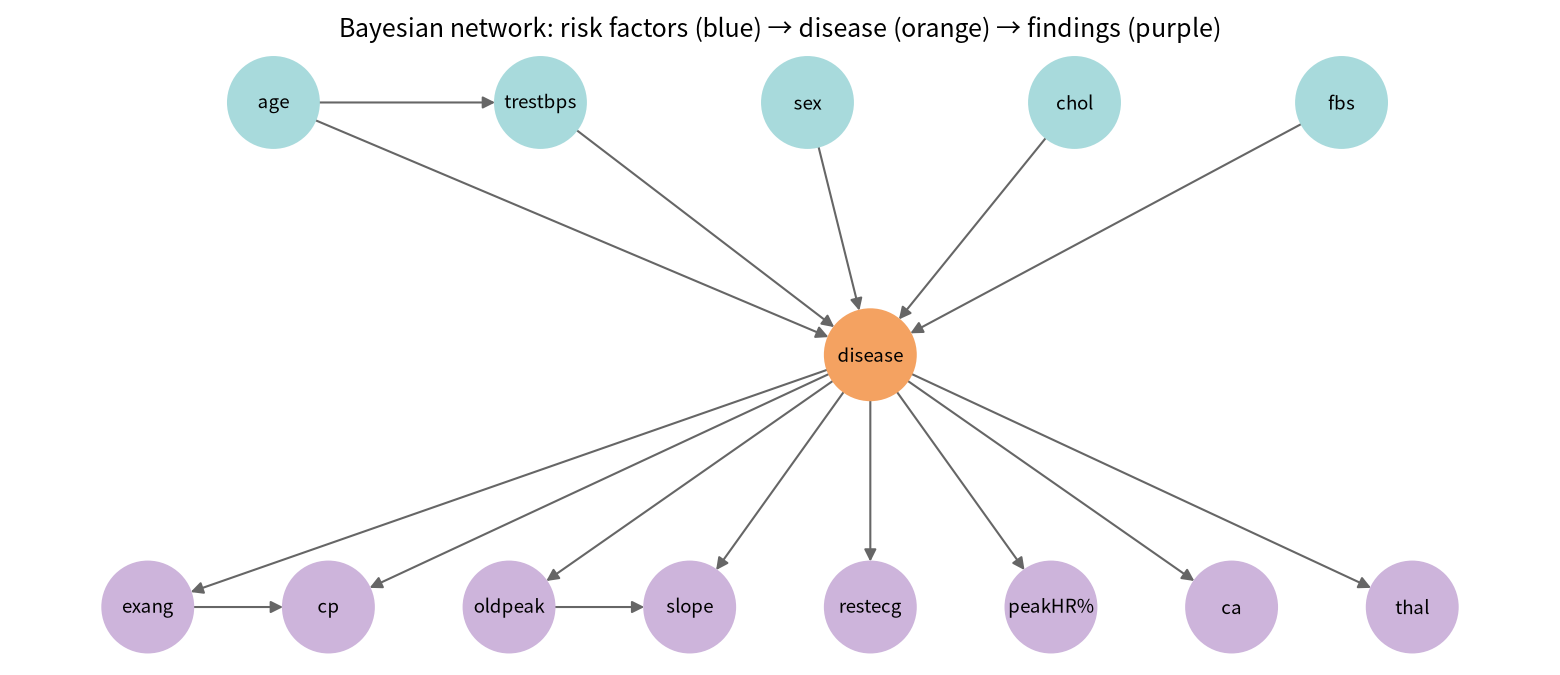
\includegraphics[width=\columnwidth]{fig_bn_structure.png}
\caption{Hand-specified network: risk factors (blue) $\rightarrow$ disease (orange) $\rightarrow$ findings (purple).}
\label{fig:bn}
\end{figure}

\subsection{Naive Bayes}
Naive Bayes is the same pipeline with the star graph $Y\rightarrow X_j$ for all $j$:
$P(Y{=}1\mid\mathbf{x})\propto P(Y{=}1)\prod_j P(x_j\mid Y{=}1)$. It assumes the predictors are conditionally independent given disease and has far fewer parameters than the BN. Whether the extra structure helps is an empirical question (H2).

\subsection{Exact additive explanation}
For a fully observed row, the Markov-blanket factorisation gives posterior log-odds
\begin{multline}
\log\frac{P(Y{=}1\mid\mathbf{x})}{P(Y{=}0\mid\mathbf{x})}
=\operatorname{logit}P\bigl(Y{=}1\mid\mathrm{pa}(Y)\bigr)\\
+\sum_{c\in\mathrm{ch}(Y)}\log\frac{P(c\mid \mathrm{pa}^{-}(c),Y{=}1)}{P(c\mid \mathrm{pa}^{-}(c),Y{=}0)},
\end{multline}
where $\mathrm{pa}^{-}(c)=\mathrm{pa}(c)\setminus\{Y\}$ is the other parents of child $c$,
i.e.\ a risk-factor term plus one weight of evidence per finding. This is exact for the model, not for physiology. It requires complete evidence: we verified agreement with pgmpy inference on all 297 complete rows (maximum absolute difference $2\times10^{-16}$); the six incomplete rows are excluded from explanations only, while predictions still use exact marginalisation.

\subsection{Classical references}
\emph{Logistic regression} uses L2 regularisation ($C=0.5$) on standardised numerics and one-hot categoricals (``continuous'') or on one-hot bins (``binned''). \emph{Random forest} \cite{breiman2001} uses 300 trees, \texttt{min\_samples\_leaf}=3, \texttt{max\_features}=$\sqrt{p}$. \emph{Prior-only} predicts the training-fold prevalence. Implementations are from scikit-learn \cite{pedregosa2011}. These settings were retained from the initial implementation and were not tuned during this project; we cannot establish that they were chosen before seeing results, and no nested cross-validation was used.

%% ------------------------------------------------------------------------------------
\section{Evaluation Protocol}
All models use the same 25 splits from \texttt{RepeatedStratifiedKFold}(5 folds, 5 repeats, seed 2026); the manifest is saved in the repository. Every patient is held out once per repeat, and all preprocessing is fitted on the training folds. Metrics are computed on the 303 out-of-fold (OOF) predictions of each repeat and then averaged over repeats. Pooling repeats for plots is descriptive: 1,515 predictions still come from 303 patients.

We report ROC AUC; AP (labelled PR AUC); sensitivity and specificity at a fixed 0.5 threshold; Brier score; ECE (10 equal-frequency bins); and the calibration slope and intercept from a logistic regression of $y$ on the logit of the OOF probability. A slope below 1 indicates over-extreme probabilities, above 1 over-compressed ones. Intervals are 95\% percentile intervals from 500 bootstrap draws of patient indices; they condition on the already-fitted OOF predictions and omit retraining variability. AUC differences are also tested with the corrected resampled $t$-test \cite{nadeau2003}. These comparisons are exploratory; no multiplicity correction is applied, and a non-significant result is not evidence of equivalence.

%% ------------------------------------------------------------------------------------
\section{Results}
\subsection{Discrimination and operating-point performance}
Table~\ref{tab:main} gives the main results. ROC AUC lies in a narrow range (0.896--0.911), and no paired AUC comparison detected a difference at the 0.05 level (Table~\ref{tab:paired}). The structured BN is not better than NB: its point estimates are lower on AUC ($-0.012$), AP ($-0.021$) and specificity. The AP interval for BN$-$NB excludes zero, but it is conditional on fixed predictions, uncorrected for multiplicity and should be read as suggestive only. Random forest is not better than logistic regression ($\Delta\mathrm{AUC}=-0.003$). On H2, therefore, we find no support in this dataset for either part; this does not show that interactions are absent, only that one forest configuration did not exploit them.

\begin{table*}[!t]
\caption{Main results: mean of five repeats of out-of-fold metrics (all models share the same 25 splits). Sensitivity and specificity at threshold 0.5. Slope is the calibration slope (ideal 1). Prior-only sensitivity/specificity are degenerate and omitted.}
\label{tab:main}
\centering
\small
\begin{tabular}{lccccccc}
\toprule
Model & ROC AUC [95\% CI] & AP & Sens. & Spec. & Brier & ECE & Slope \\
\midrule
Prior only & 0.495 & 0.456 & -- & -- & 0.248 & 0.052 & -- \\
Naive Bayes & 0.908 [0.874, 0.939] & 0.904 & 0.791 & 0.888 & 0.126 & 0.087 & 0.51 \\
Bayesian net & 0.896 [0.861, 0.927] & 0.882 & 0.778 & 0.851 & 0.139 & 0.086 & 0.49 \\
LogReg (binned) & 0.907 [0.870, 0.938] & 0.898 & 0.809 & 0.888 & 0.118 & 0.050 & 0.99 \\
LogReg (cont.) & 0.911 [0.875, 0.941] & 0.905 & 0.804 & 0.889 & 0.116 & 0.047 & 0.98 \\
Random forest & 0.908 [0.869, 0.938] & 0.901 & 0.787 & 0.855 & 0.125 & 0.055 & 1.42 \\
\bottomrule
\end{tabular}

\end{table*}

\begin{table*}[!t]
\caption{Exploratory paired comparisons (A$-$B). Intervals are paired patient bootstraps conditional on fixed predictions; $p_\mathrm{corr}$ is the corrected resampled $t$-test on fold AUCs.}
\label{tab:paired}
\centering
\small
\begin{tabular}{lcccc}
\toprule
Comparison (A $-$ B) & $\Delta$AUC [95\% CI] & $p_{\mathrm{corr}}$ & $\Delta$AP [95\% CI] & $\Delta$Brier [95\% CI] \\
\midrule
Bayesian net $-$ Naive Bayes & $-$0.012 [$-$0.026, +0.005] & 0.13 & $-$0.021 [$-$0.036, $-$0.006] & +0.013 [$-$0.002, +0.025] \\
Bayesian net $-$ LogReg (binned) & $-$0.011 [$-$0.028, +0.010] & 0.22 & $-$0.016 [$-$0.035, +0.004] & +0.021 [+0.005, +0.035] \\
Naive Bayes $-$ LogReg (cont.) & $-$0.003 [$-$0.017, +0.010] & 0.56 & $-$0.001 [$-$0.014, +0.012] & +0.010 [$-$0.002, +0.025] \\
Bayesian net $-$ LogReg (cont.) & $-$0.015 [$-$0.033, +0.005] & 0.17 & $-$0.022 [$-$0.040, $-$0.004] & +0.023 [+0.006, +0.038] \\
Random forest $-$ LogReg (cont.) & $-$0.003 [$-$0.015, +0.009] & 0.59 & $-$0.003 [$-$0.020, +0.014] & +0.009 [$-$0.000, +0.017] \\
Random forest $-$ Bayesian net & +0.012 [$-$0.008, +0.029] & 0.31 & +0.019 [$-$0.001, +0.039] & $-$0.014 [$-$0.030, +0.003] \\
LogReg (binned) $-$ LogReg (cont.) & $-$0.004 [$-$0.013, +0.004] & 0.57 & $-$0.006 [$-$0.018, +0.004] & +0.002 [$-$0.004, +0.008] \\
\bottomrule
\end{tabular}

\end{table*}

\begin{figure}[!t]
\centering
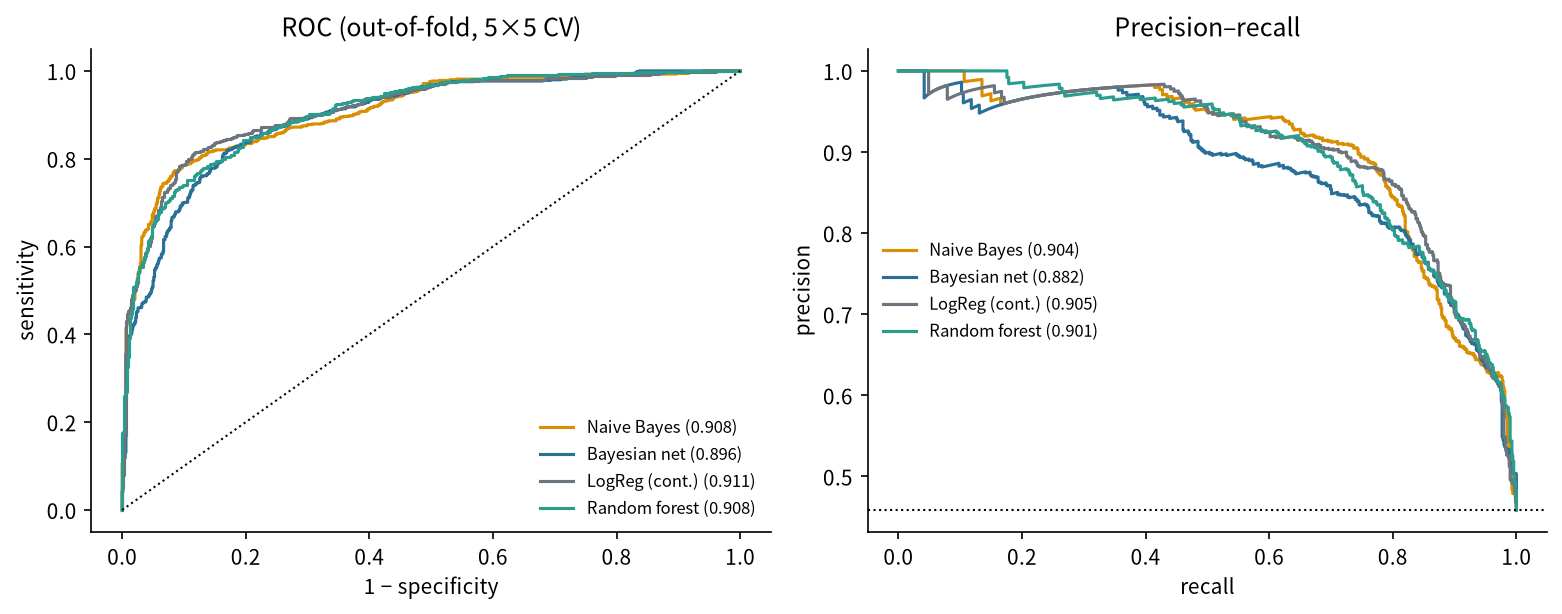
\includegraphics[width=\columnwidth]{fig_roc_pr.png}
\caption{Pooled out-of-fold ROC and precision--recall curves (descriptive; legend values are mean-per-repeat metrics).}
\label{fig:rocpr}
\end{figure}

\subsection{Calibration (H3)}
The clearest difference between families is probability quality (Fig.~\ref{fig:cal}). NB and the BN have slopes near 0.5 and many predictions at the extremes 0 and~1; logistic regression has slope 0.98 and the lowest Brier score (0.116); the random forest has slope 1.42, i.e.\ compressed probabilities. This agrees with earlier reports on how these model families behave \cite{niculescu2005}. H3 is supported in this dataset. Calibration metrics are noisy at $n=303$ (ECE is bin-sensitive) and no recalibration was fitted. Brier is overall probability loss, not a pure calibration measure.

\begin{figure*}[!t]
\centering
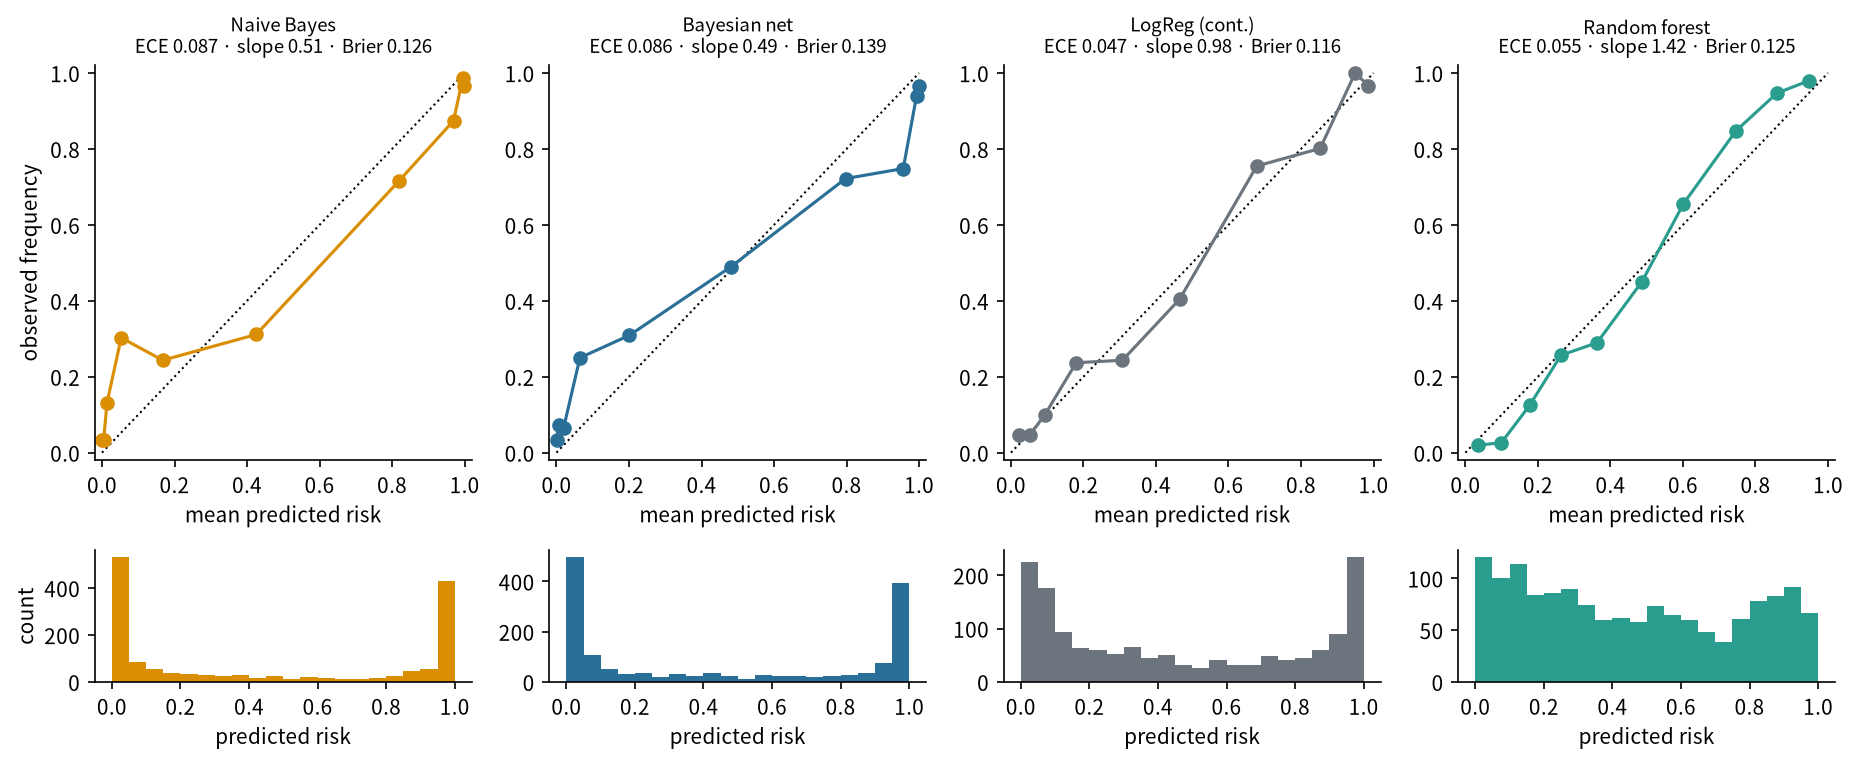
\includegraphics[width=0.9\textwidth]{fig_calibration.png}
\caption{Reliability curves (top) and predicted-risk histograms (bottom), pooled across repeats for visualisation only. ECE, slope and Brier in the panel titles are averaged per repeat.}
\label{fig:cal}
\end{figure*}

\subsection{Is binning harmful? (H1)}
The raw comparison of binned logistic regression (0.907) with continuous logistic regression (0.911) is confounded: the continuous model uses raw \texttt{thalach}, the binned one uses the age-adjusted ratio. We therefore added a continuous model with the same $\mathrm{apmhr}$ feature (Table~\ref{tab:matched}). Binned minus matched-continuous AUC is $-0.0038$ (interval $[-0.0125,+0.0043]$, corrected $p=0.62$). We therefore find no evidence in this dataset that binning costs ranking performance, so H1 is not supported here; the interval is compatible with a small loss, and the result should not be generalised. Notably, on \emph{identical binned inputs} the BN has a higher Brier score than logistic regression ($+0.021$, $[+0.005,+0.035]$), so its weakness is associated with model form (generative factorisation) rather than with binning.

\begin{table*}[!t]
\caption{Matched-input control for H1 (logistic regression)}
\label{tab:matched}
\centering
\small
\begin{tabular}{lcccc}
\toprule
Logistic regression input & ROC AUC [95\% CI] & AP & Brier & Slope \\
\midrule
Continuous, raw max HR (baseline) & 0.911 [0.875, 0.941] & 0.905 & 0.116 & 0.98 \\
Continuous, HR ratio (matched) & 0.911 [0.875, 0.941] & 0.904 & 0.116 & 0.98 \\
Binned (all numerics) & 0.907 [0.870, 0.938] & 0.898 & 0.118 & 0.99 \\
\bottomrule
\end{tabular}

\end{table*}

\subsection{Robustness}
\textbf{Dropping \texttt{ca} and \texttt{thal}} (two diagnostic work-up variables) lowers every model's AUC by 0.04--0.05 (Table~\ref{tab:noca}); the BN remains over-confident (slope 0.49). Exercise-test variables remain, so this is still not a future-risk model. \textbf{Prior strength:} varying the BDeu equivalent sample size over $\{1,5,20\}$ raises the BN slope only from 0.41 to 0.58 (Table~\ref{tab:ess}, Fig.~\ref{fig:abl}); ESS $=5$ remains the headline setting retained from the initial implementation and we do not select the best value as an unbiased winner.

\begin{table*}[!t]
\caption{Models fitted without \texttt{ca} and \texttt{thal} (same 25 splits)}
\label{tab:noca}
\centering
\small
\begin{tabular}{lccccc}
\toprule
Model & AUC (13 feat.) & AUC without ca, thal [95\% CI] & $\Delta$AUC & Brier & Slope \\
\midrule
Naive Bayes & 0.908 & 0.866 [0.825, 0.906] & $-$0.042 & 0.158 & 0.52 \\
Bayesian net & 0.896 & 0.846 [0.805, 0.884] & $-$0.050 & 0.170 & 0.49 \\
LogReg (cont.) & 0.911 & 0.872 [0.830, 0.909] & $-$0.039 & 0.144 & 0.94 \\
Random forest & 0.908 & 0.862 [0.820, 0.900] & $-$0.046 & 0.151 & 1.21 \\
\bottomrule
\end{tabular}

\end{table*}

\begin{table}[!t]
\caption{BDeu equivalent sample size sensitivity}
\label{tab:ess}
\centering
\footnotesize
\begin{tabular}{lccccc}
\toprule
Variant & ROC AUC & AP & Brier & ECE & Slope \\
\midrule
BN ESS $=$ 1 & 0.883 & 0.865 & 0.153 & 0.103 & 0.41 \\
NB ESS $=$ 1 & 0.907 & 0.902 & 0.128 & 0.088 & 0.49 \\
BN ESS $=$ 5 & 0.896 & 0.882 & 0.139 & 0.086 & 0.49 \\
NB ESS $=$ 5 & 0.908 & 0.904 & 0.126 & 0.087 & 0.51 \\
BN ESS $=$ 20 & 0.905 & 0.893 & 0.128 & 0.070 & 0.58 \\
NB ESS $=$ 20 & 0.909 & 0.906 & 0.123 & 0.080 & 0.56 \\
\bottomrule
\end{tabular}

\end{table}

\begin{figure}[!t]
\centering
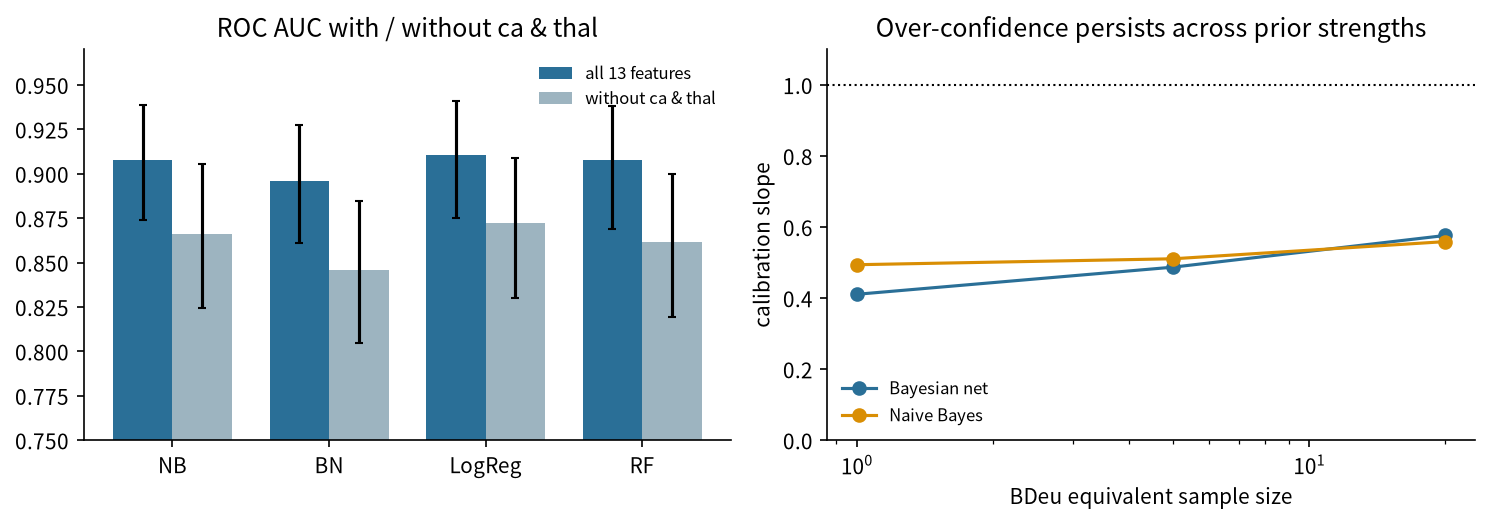
\includegraphics[width=\columnwidth]{fig_ablation.png}
\caption{Left: AUC with and without \texttt{ca}, \texttt{thal}. Right: calibration slope versus BDeu prior strength.}
\label{fig:abl}
\end{figure}

\subsection{Reading the Bayesian network}
The explanation of Eq.~(3) (Fig.~\ref{fig:w}) shows the risk-factor block, \texttt{thal} and \texttt{ca} carrying the largest mean absolute evidence. The largest false alarm (patient 252, no disease, $P=1.00$) accumulates positive terms from several findings (peak heart rate 1.9, \texttt{exang} 1.25, \texttt{thal} 1.22 in log-odds) on top of a positive risk-factor term. This is consistent with findings being combined as if independent, but sparse tables and misspecified dependencies are only plausible explanations; we did not test them. The five-variable risk-factor block is not directly comparable to a single-feature term.

\begin{figure*}[!t]
\centering
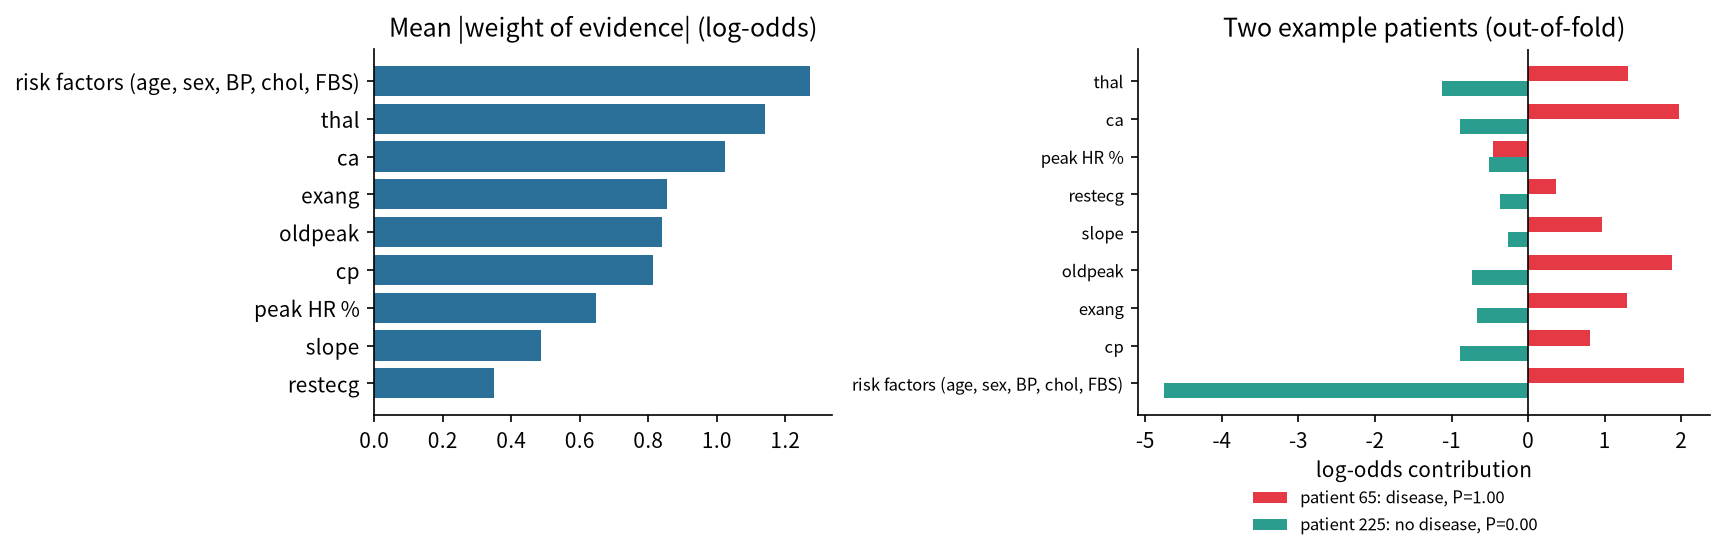
\includegraphics[width=0.85\textwidth]{fig_bn_weights.png}
\caption{Left: mean absolute weight of evidence (complete-evidence OOF rows). Right: two example patients. Units are log-odds; contributions describe the model, not causal importance.}
\label{fig:w}
\end{figure*}

%% ------------------------------------------------------------------------------------
\section{Discussion and Limitations}
\textbf{Takeaways.} (i) Ranking is similar across these classical models. (ii) Extra hand-specified structure did not help here, and generative models were less well calibrated than discriminative ones. (iii) A fair comparison needed a matched control; the raw one confounded two changes. (iv) Calibration should be assessed whenever a probability is the product, which sets the bar for the Phase~2 network: it should be compared on the same splits, with calibration reported alongside AUC \cite{guo2017}.

\textbf{Limitations.} 303 historical, single-centre, mostly male rows, with no external validation; transportability is unknown. Patient independence is assumed. The target is existing disease, and \texttt{ca}/\texttt{thal} are work-up results. The graph, cut points and heart-rate transform were EDA-informed and hyperparameters were not tuned under nested CV, so optimism is possible. Bootstrap intervals omit training variability; ECE and slope are noisy; repeated predictions are dependent; comparisons are exploratory without multiplicity control. Calibration is measured, not corrected. We make no causal claim and no claim of clinical utility.

%% ------------------------------------------------------------------------------------
\section{Reproducibility, Phase~2 and Disclosure}
Code, split manifest, predictions, metrics and a 26-test suite are in the project repository; the tables in this report are generated from \texttt{results/*.csv} by \texttt{src/build\_latex\_tables.py}. Use Python 3.12 and \texttt{requirements.txt}.

\textbf{Phase~2 plan} (not implemented here): a regularised feed-forward MLP on standardised numerics and one-hot categoricals, with preprocessing, tuning and early stopping restricted to training data; evaluation on the saved splits against the baselines in Table~\ref{tab:main}, with calibration and, optionally, SHAP \cite{lundberg2017} compared with the BN evidence weights. Because these folds have already informed Phase~1 design, any new comparison is optimistic.

\textbf{Disclosure.} AI tools (Claude, Anthropic) were used to help draft code, analysis and this report; the team is responsible for its contents. Individual contributions are recorded in the repository history and \texttt{docs/CONTRIBUTIONS.md}.

\bibliographystyle{IEEEtran}
\bibliography{references}

\end{document}
